\documentclass{beamer}
%\usetheme{}%\usecolortheme{}
\setbeamertemplate{navigation symbols}{}
\setbeamertemplate{section in toc}[sections numbered]
\setbeamertemplate{footline}[frame number]

\usepackage[utf8]{inputenc}
\usepackage[T1]{fontenc}
\usepackage{lmodern}
\usepackage{appendixnumberbeamer}
\usepackage{multirow}

\title{%
  \textbf{BEST: a Binary Executable Slicing Tool}
  \\ and its use to improve
  \\ Model Checking-based WCET Analysis}
\author{%
  \textbf{Armel Mangean}$^1$
  \and Jean-Luc Béchennec$^2$
  \and Mikaël Briday$^3$
  \and Sébastien Faucou$^3$}
\institute{%
  IRCCyN, UMR CNRS 6597
  \\ $^1$École Centrale de Nantes, $^2$CNRS , $^3$Université de Nantes}
\date{July 5, 2016}

% 20 min -> ~15 slides

\begin{document}

  \begin{frame}
    \titlepage

    \begin{center}
      
\includegraphics[height=0.8cm]{fig/irccyn.png}
    \end{center}

    \emph{\small 16th International Workshop on Worst-Case Execution Time Analysis}
  \end{frame}

  \begin{frame}
    \frametitle{~}
    \tableofcontents
  \end{frame}

  %%%
  
  \section{Introduction}
  \begin{frame}
    \frametitle{\secname}
    \tableofcontents[currentsection]
  \end{frame}
  
  \subsection{Motivation}
  \begin{frame}
    \frametitle{\secname}
    \framesubtitle{\subsecname}
    
    \begin{figure}
      \centering
      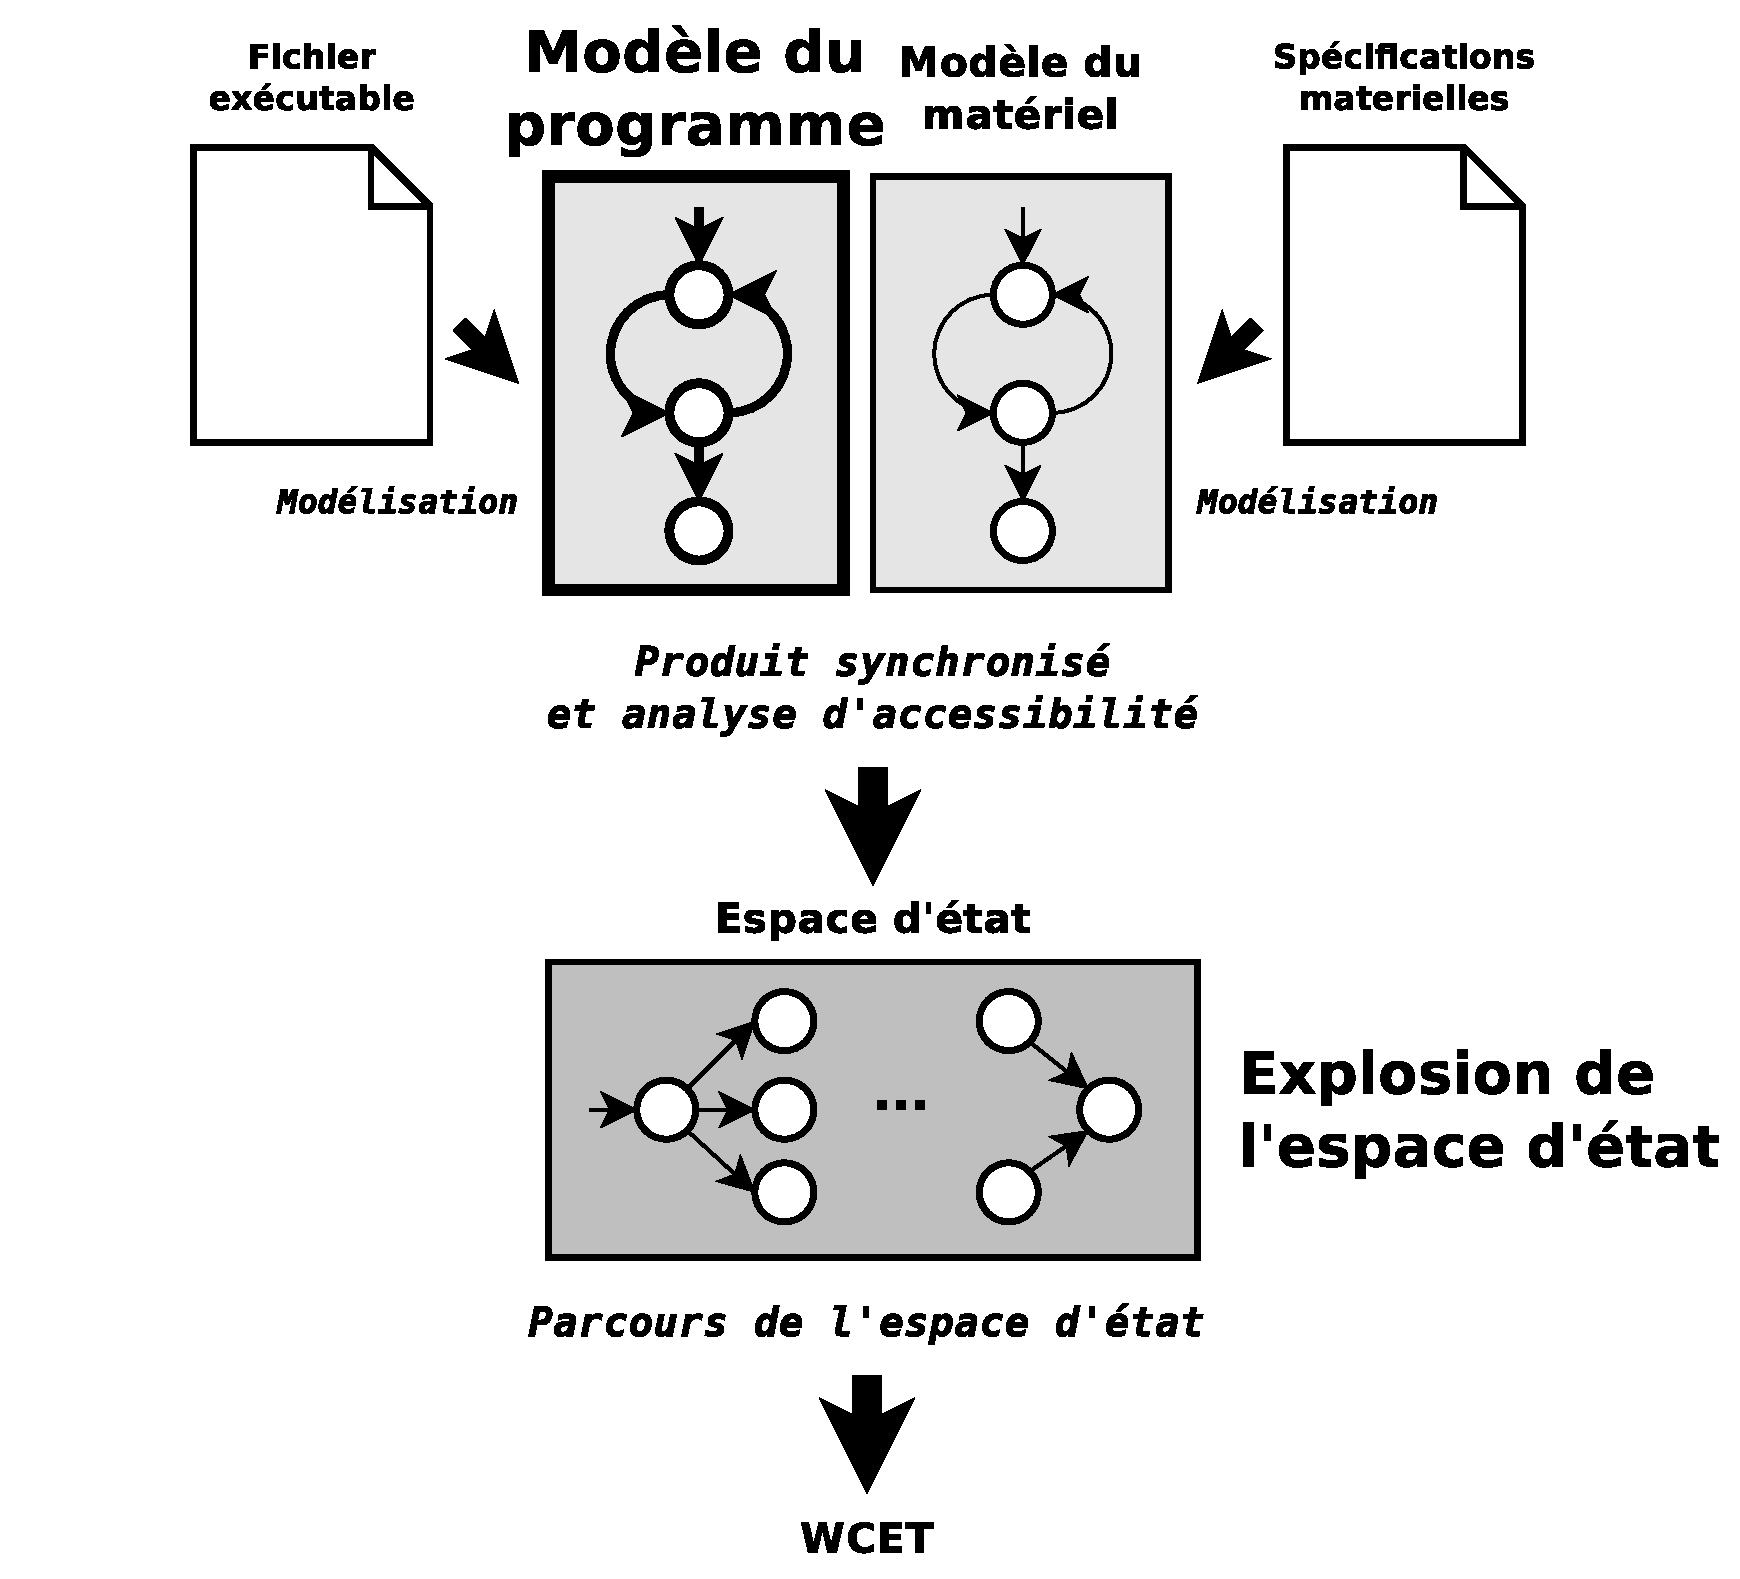
\includegraphics[height=.85\textheight]{fig/model-checking.eps}
    \end{figure}
  \end{frame}

  \begin{frame}
    \frametitle{\secname}
    \framesubtitle{\subsecname}
    
    \begin{block}{Motivation:}
        \begin{description}
          \item[modularity] network of timed automata
          \item[tightness] exact cache analysis
            \begin{itemize} % infeasible with AI
            \item arbitrary cache policy (not only LRU nor PLRU)
            \end{itemize}

          \vspace{1em}
          \item[witnesses] initial hardware and software states
          \item[binary level] no high level source code analysis
        \end{description}
    \end{block}
  \end{frame}
  
  \subsection{Challenge}
  \begin{frame}
    \frametitle{\secname}
    \framesubtitle{\subsecname}
      
    \begin{block}{Limitations:}
      \begin{itemize}
        \item suffer of the state space explosion
        \item tailored for embedded microcontrollers % but thus precise
      \end{itemize}
    \end{block}
    
    \vspace{1em}
    \begin{block}{Challenges:}
      \begin{itemize}
        \item abstracting models of hardware components~\cite{CGM15}
        \item \textbf{abstracting models of programs}~\cite{BJ14,CB13,MBB16}
      \end{itemize}
    \end{block}
  \end{frame}

  %%%

  \section{Program Abstraction using Program Slicing}
  \begin{frame}
    \frametitle{\secname}
    \tableofcontents[currentsection]
  \end{frame}

  \subsection{Overview of Program Slicing}
  \begin{frame}
    \frametitle{\secname}
    \framesubtitle{\subsecname}

    \begin{itemize}
      \item a program $P \subseteq L \times I$ with
        \begin{itemize}
          \item $L$ a finite set of labels
          \item $I$ a finite set of instructions
          \item $\forall (l,i), (l,i') \in P, i = i'$
        \end{itemize}
      \item $V_P$ the finite set of variables of $P$

      \vspace{1em}
      \item introduced by Weiser in 1981~\cite{Wei81}
      \item a criterion $C = (l,v)$ with
        \begin{itemize}
          \item $l \in L$ a label and
          \item $v \in V_P$ a subset of variables
        \end{itemize}
      \item a slice $S_C \subseteq P$
        \begin{itemize}
          \item same behavior as $P$ wrt. criterion $C$
        \end{itemize}
    \end{itemize}
  \end{frame}
  
  \begin{frame}
    \frametitle{\secname}
    \framesubtitle{\subsecname}

    \vspace{1em}
    \begin{figure}
      \centering
      \begin{overlayarea}{\textwidth}{\textheight}
        \only<1>{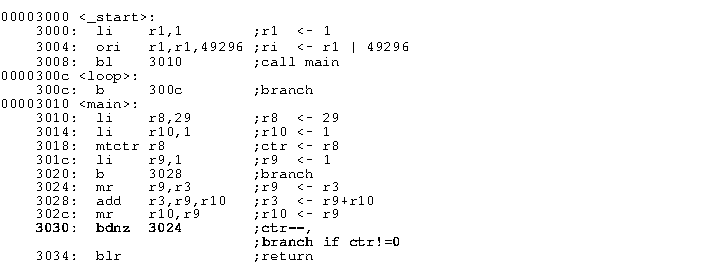
\includegraphics[scale=1.4]{fig/fibcallO2-01.pdf}}
        \only<2>{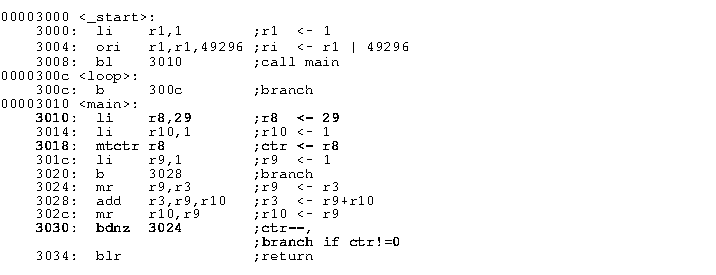
\includegraphics[scale=1.4]{fig/fibcallO2-02.pdf}}
        \begin{center}
          Slicing criterion: $C = ( 3030, \{ctr\} )$
        \end{center}
      \end{overlayarea}
    \end{figure}
  \end{frame}
  
  \begin{frame}
    \frametitle{\secname}
    \framesubtitle{\subsecname}
    
    \begin{itemize}
      \item dataflow equation-based or graph-based
        \begin{itemize}
          \item fixpoint computation or
          \item reachability analysis
        \end{itemize}
        
      \vspace{1em}
      \item slicing binary executables
      \begin{itemize}
        \item a closed issue~\cite{KJL03} (although not trivial)
        \item multiple graph computation from a CFG
        \item reachability analysis on the final graph
      \end{itemize}
      
      %% \vspace{1em}
      %% \item intuition
      %% \begin{itemize}
      %%   \item the Control Flow Graph
      %%   \item a Control Dependence Graph (of basic blocks)
      %%   \item a Data Dependence Graph (of instructions)
      %%   \item a summary Program Dependence Graph
      %% \end{itemize}
    \end{itemize}
  \end{frame}
  

  \subsection{Abstracting models of programs}
  \begin{frame}
    \frametitle{\secname}
    \framesubtitle{\subsecname}

    \begin{figure}
      \centering
      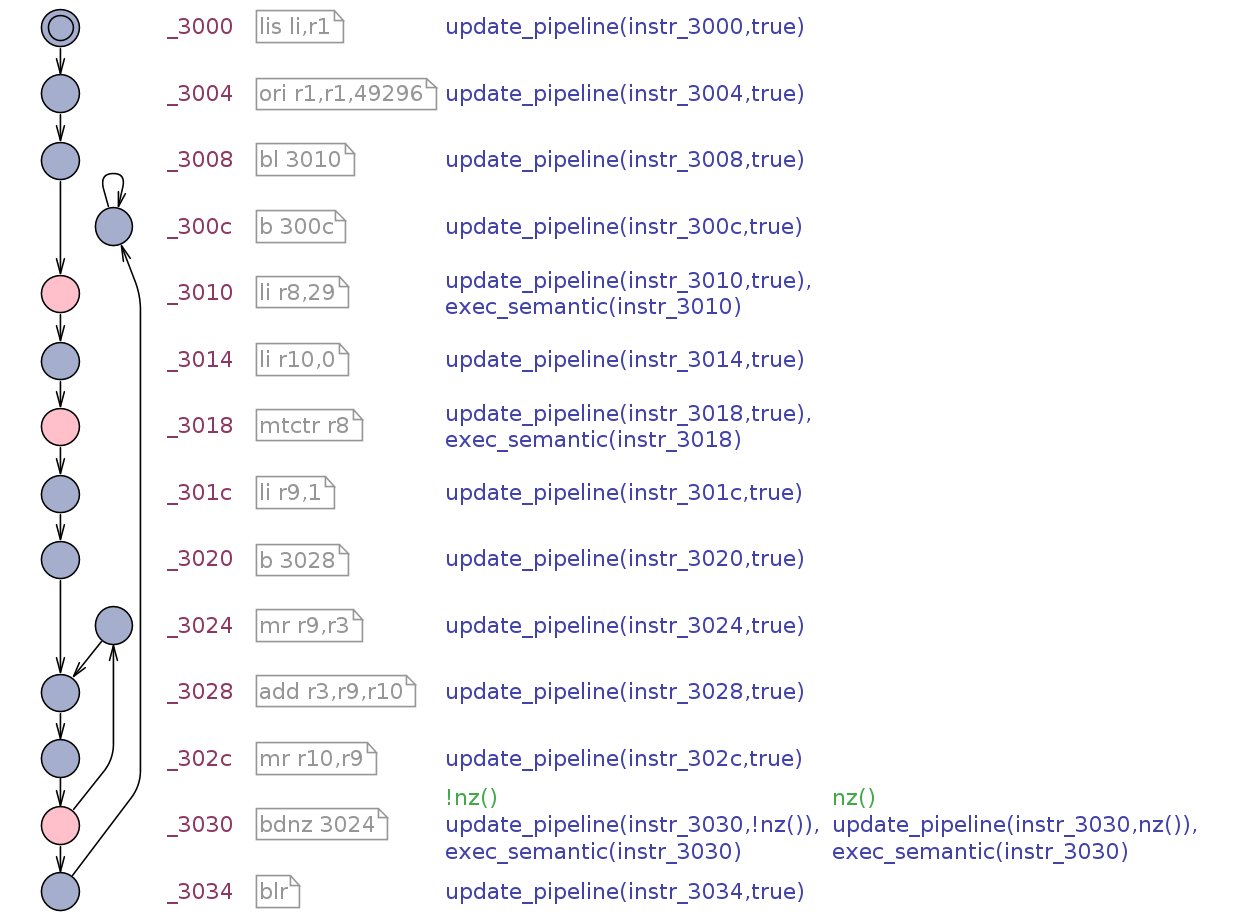
\includegraphics[height=.85\textheight]{fig/example.png}
    \end{figure}

    %% \begin{itemize}
    %%   \item how to abstract models of program using program slicing?
    %%   \item removing instructions would results in losing essential information
    %%     regarding registers use and thus pipeline timing behavior.
    %%   \item so we can't remove instructions

    %%   \item what can we remove?
        
    %%   \item How do we use Program Slicing to abstract models of programs?
      
    %%   \vspace{1em}
    %%   \item Abstracted models of programs keep the same time behaviour as
    %%     unabstracted models.
    %%   \item We do not intend to perform WCET analysis on slices but on abstracts
    %%     models of programs built using information gathered through program
    %%     slicing.
    %%   \item Instructions not in the slice are abstracted (not removed, they keep
    %%     their time behaviour) others are not.
    %% \end{itemize}
  \end{frame}

  \subsection{Tool implementation}
  \begin{frame}
    \frametitle{\secname}
    \framesubtitle{\subsecname}

    \begin{figure}
      \centering
      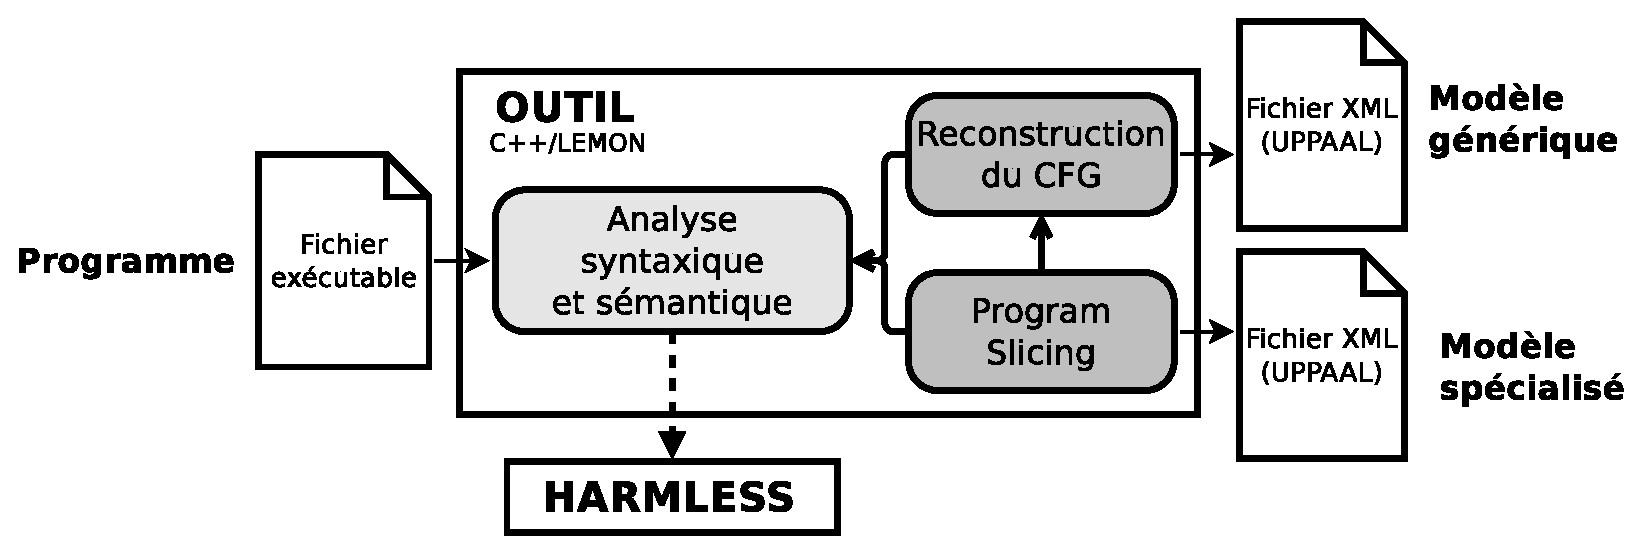
\includegraphics[height=.85\textheight]{fig/archi.eps}
    \end{figure}
  \end{frame}

  %%%
  
  \section{Experimental results}
  \begin{frame}
    \frametitle{\secname}
    \tableofcontents[currentsection]
  \end{frame}
  
  \subsection{Methodology}
  \begin{frame}
    \frametitle{\secname}
    \framesubtitle{\subsecname}

    \begin{itemize}
      \item use of Mälardalen WCET benchmarks
      \item excluding programs containing % 16 out of the 35
        \begin{itemize}
          \item switch-case statements % whereas it's a closed issue
          \item floating-point arithmetic % missing in the PowerPC HADL file 
          \item recursive programs
        \end{itemize}
      \item multiple compilers and optimisation options
        \begin{itemize}
          \item \textsc{Gcc} 5.3.1 (\texttt{-O0}, \texttt{-O1}, \texttt{-O2}, \texttt{-O3})
          \item \textsc{Cosmic C} 4.3.7 (\texttt{-no}, \emph{default})
          \item targeting the PowerPC 32 bits instruction set
        \end{itemize}
      \item sums up to 96 binaries

      \vspace{1em}
      \item use of Trampoline RTOS~\cite{BBF06} services
        \begin{itemize}
          \item not documented on our paper
        \end{itemize}
    \end{itemize}
  \end{frame}
  
  \subsection{Results}
  \begin{frame}
    \frametitle{\secname}
    \framesubtitle{\subsecname}

    \begin{table}
      \centering
      \tiny
      %!TEX root = ./main.tex
\section{Experimental results}
\label{sec:results}

  % TODO: (2 pages)
  % - Que veut-on mesurer ?
  % - Définition et justification de notre métrique
  % - Tableaux de résultats et description
  % - Analyse et recul

  We have conducted experiments to measure the reduction of the set of memory
  locations that must be included in the model. Given the current restriction of
  \best{}, we have focused on the registers. To do so, \best\ outputs the
  following information for each program:
  \begin{itemize}
    \item the number of registers used either explicitly or implicitly and the
      number of instructions in the original program ;
    \item the number of registers used either explicitly or implicitly and the
      number of instructions in the sliced program (using the slicing criterion
      defined in Section~\ref{sec:slicing}).
  \end{itemize}
 
  %. For
  %each benchmark we have counted the number $\alpha$ of explicitly and
  %implicitly used registers in the binary executable file. These registers are
  %either from the 32 general purpose registers ($r0$, $r1$, dots, $r32$) or from
  %the 5 dedicated registers ($cr$, $xer$, $lr$, $ctr$, $pc$). Then, we have
  %counted the number $\beta$ of explicitly and implicitly used registers in the
  %slice of the binary executable file according to our specific slicing criteria
  %(see subsection~\ref{subsec:slicing-reduction}). Lastly, we have computed the
  %reduction rate $\gamma = (\alpha - \beta) / \alpha$.

  We used the Mälardalen WCET benchmarks~\cite{Gustafsson:WCET2010:Benchmarks}
  to generate the programs. We had to exclude certain programs to account for the
  current limitation of our tool: program containing floating point arithmetic
  or switch-case statements and recursive programs.

  We used the library generated by the \h\ compiler from a description of a
  PowerPC e200z4 core based on the 32 bits PowerPC instruction set. This
  architecture includes 32 general purpose registers ($r0$, $r1$, \ldots, $r31$)
  and 5 dedicated registers ($cr$, $xer$, $lr$, $ctr$, $pc$). We used two
  different compilers: \gcc\ $5.3.1$ and \cosmic\ $4.3.7$. For a given compiler,
  the generated binary may be very different according to the optimizations. For
  instance without optimization \gcc\ generates code where local variables are
  loaded from and stored to the stack frame each time they are used, whereas in
  higher optimization levels local variables are allocated in registers. Thus we
  created different program versions for each optimization level offered by each
  compiler (4 levels for \gcc\ and 2 levels for \cosmic{}).
  
  All in all, we created 6 versions of each of the 16 Mälardalen benchmarks
  fitting our constraints and we ran \best\ on these 96 programs. Due to space
  limitations the detailed results are provided online\footnote{available at
    \url{https://github.com/TrampolineRTOS/BEST}}. The results are summarized in
  Table~\ref{tab:recap} and~\ref{tab:reginslice}. Table~\ref{tab:recap} gives
  the ratio of registers and instructions in the slice compared to the original
  program. Table~\ref{tab:reginslice} gives the number of registers in the
  slice. It is not meaningful to compare our results with pior work~\cite{CB13}
  because we consider a different instruction set and different compilers (or at
  least compiler version for~\textsc{Gcc}). We do not comment either on the
  execution time of \best\ that were below one second in every case.
  
  \begin{table}
      \centering
      \resizebox{\columnwidth}{!}{%
          \begin{tabular}{|c|c| |c|c|c|c||c|c|c|c|}
   \hline
   \multirow{2}{*}{Compiler} & \multirow{2}*{Optim.} & \multicolumn{4}{c||}{Registers in slice} & \multicolumn{4}{c|}{Instructions in slice} 
   \\\cline{3-10}
    & &  Avg. & Min & Max. & Std. dev. &  Avg. & Min & Max. & Std. dev. 

    \\\hline\hline
    \multirow{4}{*}{\textsc{Gcc}} & \verb|-O0| & 61.8\% & 43.7\%  & 78.9\% & 8.8\% & 21.6\% & 1.7\% & 43.2\% & 8.9\%
    
    \\\cline{2-10}
     & \verb|-O1| & 64.6\% & 19.1\%  & 87.5\% & 13.6\% & 36.7\% & 3.24\% & 67.9\% & 10.2\%
    
    \\\cline{2-10}
     & \verb|-O2| & 64.3\% & 13.3\%  & 92.9\% & 20.3\% & 37.8\% & 2.9\% & 72.5\% & 15.7\%
    
    \\\cline{2-10}
     & \verb|-O3| & 62.8\% & 9\%  & 96.4\% & 21.7\% & 34.7\% & 0.4\% & 72.2\% & 18\%


     \\\hline\hline
     \multirow{2}*{\textsc{Cosmic C}} & \verb|-no| & 40.5\% & 8.6\% & 86.7\% & 16.6\% & 34\% & 1.9\% & 60.2\% & 15.2\% 
    
     \\\cline{2-10}
     & \emph{default} & 37\% & 2.8\% & 66.7\% & 15.8\% & 37\% & 2.8\% & 66.7\% & 15.8\% 
  
     \\\hline
\end{tabular}

%
      }
      \caption{\centering Ratio of registers (resp. instructions) in slice compared to the unsliced program.% \\
      }
      \label{tab:recap}
  \end{table}

  \begin{table}
      \centering
      %\resizebox{.55\columnwidth}{!}{%
      
\begin{tabular}{|c|c|c|c||c|c|}
   \hline
    \multicolumn{4}{|c||}{\textsc{Gcc}} & \multicolumn{2}{c|}{\textsc{Cosmic}} 
    
    \\\hline

    \verb|-O0| & \verb|-O1| &\verb|-O2| &\verb|-O3| & \verb|-no| & \emph{default}

    \\\hline

    8.8 & 13 & 11.8 & 12.1 & 11.9 & 12
  
     \\\hline
\end{tabular}
%
      %}
      \caption{\centering Average number of registers in slice.% \\
      }
      \label{tab:reginslice}
  \end{table}

  
  These results confirm that slicing is an effective abstraction technique for
  our use case.  It allows a significant reduction of the number of variables
  that should be included in the model (reduction of the dimension of the state
  space) as well as the number of instructions the output of which should be
  taken into account (reduction of the number of states to explore).  As
  expected, the best results are obtained for programs with very simple control
  flow, namely \verb|fdct.c| and \verb|jfdctint.c|, whereas the worst results
  are obtained for programs with nested control statements and procedure calls ,
  namely \verb|ndes.c| and \verb|adpcm.c|. However, let us underline that the
  structure of the source code is not always the dominant factor.  For some
  programs, it appears that the compiler (version and/or optimization) has more
  impact on the capacity of the program slicer to abstract the binary. Example
  of such programs are \verb|expint.c| and \verb|fir.c|.

  %% \todo{AM}{Jette un oeil à ces progs. pour voir si tu trouves une
  %% explication}.

   

  
  %\begin{table}
    %\centering
    %\resizebox{.8\columnwidth}{!}{%
    %%!TEX root = ./main.tex
\section{Experimental results}
\label{sec:results}

  % TODO: (2 pages)
  % - Que veut-on mesurer ?
  % - Définition et justification de notre métrique
  % - Tableaux de résultats et description
  % - Analyse et recul

  We have conducted experiments to measure the reduction of the set of memory
  locations that must be included in the model. Given the current restriction of
  \best{}, we have focused on the registers. To do so, \best\ outputs the
  following information for each program:
  \begin{itemize}
    \item the number of registers used either explicitly or implicitly and the
      number of instructions in the original program ;
    \item the number of registers used either explicitly or implicitly and the
      number of instructions in the sliced program (using the slicing criterion
      defined in Section~\ref{sec:slicing}).
  \end{itemize}
 
  %. For
  %each benchmark we have counted the number $\alpha$ of explicitly and
  %implicitly used registers in the binary executable file. These registers are
  %either from the 32 general purpose registers ($r0$, $r1$, dots, $r32$) or from
  %the 5 dedicated registers ($cr$, $xer$, $lr$, $ctr$, $pc$). Then, we have
  %counted the number $\beta$ of explicitly and implicitly used registers in the
  %slice of the binary executable file according to our specific slicing criteria
  %(see subsection~\ref{subsec:slicing-reduction}). Lastly, we have computed the
  %reduction rate $\gamma = (\alpha - \beta) / \alpha$.

  We used the Mälardalen WCET benchmarks~\cite{Gustafsson:WCET2010:Benchmarks}
  to generate the programs. We had to exclude certain programs to account for the
  current limitation of our tool: program containing floating point arithmetic
  or switch-case statements and recursive programs.

  We used the library generated by the \h\ compiler from a description of a
  PowerPC e200z4 core based on the 32 bits PowerPC instruction set. This
  architecture includes 32 general purpose registers ($r0$, $r1$, \ldots, $r31$)
  and 5 dedicated registers ($cr$, $xer$, $lr$, $ctr$, $pc$). We used two
  different compilers: \gcc\ $5.3.1$ and \cosmic\ $4.3.7$. For a given compiler,
  the generated binary may be very different according to the optimizations. For
  instance without optimization \gcc\ generates code where local variables are
  loaded from and stored to the stack frame each time they are used, whereas in
  higher optimization levels local variables are allocated in registers. Thus we
  created different program versions for each optimization level offered by each
  compiler (4 levels for \gcc\ and 2 levels for \cosmic{}).
  
  All in all, we created 6 versions of each of the 16 Mälardalen benchmarks
  fitting our constraints and we ran \best\ on these 96 programs. Due to space
  limitations the detailed results are provided online\footnote{available at
    \url{https://github.com/TrampolineRTOS/BEST}}. The results are summarized in
  Table~\ref{tab:recap} and~\ref{tab:reginslice}. Table~\ref{tab:recap} gives
  the ratio of registers and instructions in the slice compared to the original
  program. Table~\ref{tab:reginslice} gives the number of registers in the
  slice. It is not meaningful to compare our results with pior work~\cite{CB13}
  because we consider a different instruction set and different compilers (or at
  least compiler version for~\textsc{Gcc}). We do not comment either on the
  execution time of \best\ that were below one second in every case.
  
  \begin{table}
      \centering
      \resizebox{\columnwidth}{!}{%
          \begin{tabular}{|c|c| |c|c|c|c||c|c|c|c|}
   \hline
   \multirow{2}{*}{Compiler} & \multirow{2}*{Optim.} & \multicolumn{4}{c||}{Registers in slice} & \multicolumn{4}{c|}{Instructions in slice} 
   \\\cline{3-10}
    & &  Avg. & Min & Max. & Std. dev. &  Avg. & Min & Max. & Std. dev. 

    \\\hline\hline
    \multirow{4}{*}{\textsc{Gcc}} & \verb|-O0| & 61.8\% & 43.7\%  & 78.9\% & 8.8\% & 21.6\% & 1.7\% & 43.2\% & 8.9\%
    
    \\\cline{2-10}
     & \verb|-O1| & 64.6\% & 19.1\%  & 87.5\% & 13.6\% & 36.7\% & 3.24\% & 67.9\% & 10.2\%
    
    \\\cline{2-10}
     & \verb|-O2| & 64.3\% & 13.3\%  & 92.9\% & 20.3\% & 37.8\% & 2.9\% & 72.5\% & 15.7\%
    
    \\\cline{2-10}
     & \verb|-O3| & 62.8\% & 9\%  & 96.4\% & 21.7\% & 34.7\% & 0.4\% & 72.2\% & 18\%


     \\\hline\hline
     \multirow{2}*{\textsc{Cosmic C}} & \verb|-no| & 40.5\% & 8.6\% & 86.7\% & 16.6\% & 34\% & 1.9\% & 60.2\% & 15.2\% 
    
     \\\cline{2-10}
     & \emph{default} & 37\% & 2.8\% & 66.7\% & 15.8\% & 37\% & 2.8\% & 66.7\% & 15.8\% 
  
     \\\hline
\end{tabular}

%
      }
      \caption{\centering Ratio of registers (resp. instructions) in slice compared to the unsliced program.% \\
      }
      \label{tab:recap}
  \end{table}

  \begin{table}
      \centering
      %\resizebox{.55\columnwidth}{!}{%
      
\begin{tabular}{|c|c|c|c||c|c|}
   \hline
    \multicolumn{4}{|c||}{\textsc{Gcc}} & \multicolumn{2}{c|}{\textsc{Cosmic}} 
    
    \\\hline

    \verb|-O0| & \verb|-O1| &\verb|-O2| &\verb|-O3| & \verb|-no| & \emph{default}

    \\\hline

    8.8 & 13 & 11.8 & 12.1 & 11.9 & 12
  
     \\\hline
\end{tabular}
%
      %}
      \caption{\centering Average number of registers in slice.% \\
      }
      \label{tab:reginslice}
  \end{table}

  
  These results confirm that slicing is an effective abstraction technique for
  our use case.  It allows a significant reduction of the number of variables
  that should be included in the model (reduction of the dimension of the state
  space) as well as the number of instructions the output of which should be
  taken into account (reduction of the number of states to explore).  As
  expected, the best results are obtained for programs with very simple control
  flow, namely \verb|fdct.c| and \verb|jfdctint.c|, whereas the worst results
  are obtained for programs with nested control statements and procedure calls ,
  namely \verb|ndes.c| and \verb|adpcm.c|. However, let us underline that the
  structure of the source code is not always the dominant factor.  For some
  programs, it appears that the compiler (version and/or optimization) has more
  impact on the capacity of the program slicer to abstract the binary. Example
  of such programs are \verb|expint.c| and \verb|fir.c|.

  %% \todo{AM}{Jette un oeil à ces progs. pour voir si tu trouves une
  %% explication}.

   

  
  %\begin{table}
    %\centering
    %\resizebox{.8\columnwidth}{!}{%
    %%!TEX root = ./main.tex
\section{Experimental results}
\label{sec:results}

  % TODO: (2 pages)
  % - Que veut-on mesurer ?
  % - Définition et justification de notre métrique
  % - Tableaux de résultats et description
  % - Analyse et recul

  We have conducted experiments to measure the reduction of the set of memory
  locations that must be included in the model. Given the current restriction of
  \best{}, we have focused on the registers. To do so, \best\ outputs the
  following information for each program:
  \begin{itemize}
    \item the number of registers used either explicitly or implicitly and the
      number of instructions in the original program ;
    \item the number of registers used either explicitly or implicitly and the
      number of instructions in the sliced program (using the slicing criterion
      defined in Section~\ref{sec:slicing}).
  \end{itemize}
 
  %. For
  %each benchmark we have counted the number $\alpha$ of explicitly and
  %implicitly used registers in the binary executable file. These registers are
  %either from the 32 general purpose registers ($r0$, $r1$, dots, $r32$) or from
  %the 5 dedicated registers ($cr$, $xer$, $lr$, $ctr$, $pc$). Then, we have
  %counted the number $\beta$ of explicitly and implicitly used registers in the
  %slice of the binary executable file according to our specific slicing criteria
  %(see subsection~\ref{subsec:slicing-reduction}). Lastly, we have computed the
  %reduction rate $\gamma = (\alpha - \beta) / \alpha$.

  We used the Mälardalen WCET benchmarks~\cite{Gustafsson:WCET2010:Benchmarks}
  to generate the programs. We had to exclude certain programs to account for the
  current limitation of our tool: program containing floating point arithmetic
  or switch-case statements and recursive programs.

  We used the library generated by the \h\ compiler from a description of a
  PowerPC e200z4 core based on the 32 bits PowerPC instruction set. This
  architecture includes 32 general purpose registers ($r0$, $r1$, \ldots, $r31$)
  and 5 dedicated registers ($cr$, $xer$, $lr$, $ctr$, $pc$). We used two
  different compilers: \gcc\ $5.3.1$ and \cosmic\ $4.3.7$. For a given compiler,
  the generated binary may be very different according to the optimizations. For
  instance without optimization \gcc\ generates code where local variables are
  loaded from and stored to the stack frame each time they are used, whereas in
  higher optimization levels local variables are allocated in registers. Thus we
  created different program versions for each optimization level offered by each
  compiler (4 levels for \gcc\ and 2 levels for \cosmic{}).
  
  All in all, we created 6 versions of each of the 16 Mälardalen benchmarks
  fitting our constraints and we ran \best\ on these 96 programs. Due to space
  limitations the detailed results are provided online\footnote{available at
    \url{https://github.com/TrampolineRTOS/BEST}}. The results are summarized in
  Table~\ref{tab:recap} and~\ref{tab:reginslice}. Table~\ref{tab:recap} gives
  the ratio of registers and instructions in the slice compared to the original
  program. Table~\ref{tab:reginslice} gives the number of registers in the
  slice. It is not meaningful to compare our results with pior work~\cite{CB13}
  because we consider a different instruction set and different compilers (or at
  least compiler version for~\textsc{Gcc}). We do not comment either on the
  execution time of \best\ that were below one second in every case.
  
  \begin{table}
      \centering
      \resizebox{\columnwidth}{!}{%
          \input{fig/recap}%
      }
      \caption{\centering Ratio of registers (resp. instructions) in slice compared to the unsliced program.% \\
      }
      \label{tab:recap}
  \end{table}

  \begin{table}
      \centering
      %\resizebox{.55\columnwidth}{!}{%
      \input{fig/reginslice}%
      %}
      \caption{\centering Average number of registers in slice.% \\
      }
      \label{tab:reginslice}
  \end{table}

  
  These results confirm that slicing is an effective abstraction technique for
  our use case.  It allows a significant reduction of the number of variables
  that should be included in the model (reduction of the dimension of the state
  space) as well as the number of instructions the output of which should be
  taken into account (reduction of the number of states to explore).  As
  expected, the best results are obtained for programs with very simple control
  flow, namely \verb|fdct.c| and \verb|jfdctint.c|, whereas the worst results
  are obtained for programs with nested control statements and procedure calls ,
  namely \verb|ndes.c| and \verb|adpcm.c|. However, let us underline that the
  structure of the source code is not always the dominant factor.  For some
  programs, it appears that the compiler (version and/or optimization) has more
  impact on the capacity of the program slicer to abstract the binary. Example
  of such programs are \verb|expint.c| and \verb|fir.c|.

  %% \todo{AM}{Jette un oeil à ces progs. pour voir si tu trouves une
  %% explication}.

   

  
  %\begin{table}
    %\centering
    %\resizebox{.8\columnwidth}{!}{%
    %\input{fig/results}%
    %}
    %\caption{\centering Results for Mälardalen benchmark. \\
      %Results in each column are expressed as ``-$\gamma$\%~($\alpha$)''% where \\
%%      $\alpha$ is the number of explicitly and implicitly used registers in the original program ;\\
%%      $\beta$ is the number of explicitly and implicitly used registers in the slice ; \\
%%      $\gamma = (\alpha - \beta) / \alpha \times 100$, the gain in percentage.
      %\\\todo{AM}{Réexporter les données}}
    %\label{tab:results}
  %\end{table}

  
  %Overall, the average reduction is $41\%$ with a standard deviation of $24$.
  %This result \todo{AM}{Comparaison avec ACSD 13 ?}
  %It confirms the interest of the approach.
  %The average reduction is $35\%$ for \gcc\ and $55\%$ for \cosmic{}.
  %The reason is that \cosmic\ uses extensively the general purpose registers:
  %the mean value of $\alpha$ is $32$ in the case of \cosmic\ and $20$ for
  %\gcc\ ($14$ for level \texttt{O0}).
  
  %% It is thus expected that the development of the stack frame analysis will
  %% improve the results in the case of \gcc{}. \todo{AM}{Est-ce certain ?
  %% d'après tes notes, il y a moins de load /store dans gcc optim quand dans
  %% cosmic, néanmoins il y a plus de registre utilisés dans cosmic : il faut
  %% creuser cela}.

  %The worst results are obtained with \verb|ndes.c| compiled with
  %\gcc\ (\verb|-O3|) and \verb|adpcm.c| compiled with \gcc\ (\verb|-O2|). While,
  %the binaries are constituted respectively of 886 and 1094 instructions, the
  %slices are constituted of 522 and 421 instructions, i.e. 62\% and 38\% of the
  %instructions of the original program. \verb|ndes.c| and \verb|adpcm.c| do
  %extensive use of nested control statements (if-then-else statements, for-loop
  %and while-loops) and extensive use of calls to the same small procedures.

  %The best results are obtained with \verb|fdct.c| and and \verb|jfdctint.c|
  %both compiled with \cosmic\. While, the binaries are constituted respectively
  %of 218 and 205 instructions, the slices are constituted of 6 and 9
  %instructions, i.e. 3\% and 4\% of the instructions of the original program.
  %\verb|fdct.c| and \verb|jfdctint.c| are two implementations of the same
  %algorithm. They are made of only two not-nested for-loops with extensive
  %sequential computation in both loops and no procedure call.
  
  %\todo{AM}{On se pose la question de la dépendance des résultats au programme. Pour visualiser cela simplement, on pourrait tracer la courbe de gamma en fonction du programme par compilateur (dans le papier) et par niveau d'optimisation et commenter (sur le site web uniquement).}
  

  %Not optimized binaries produced with \gcc\ does extensive use of the stack
  %with a mean of 174 loads or stores per binary. Lowering the number of memory
  %access is one of the major optimization introduced with the first optimization
  %level on \gcc\ (\verb|-O1|) with a mean of 56 loads or stores per binary.
  %Whereas, not optimized binaries produces with \cosmic\ (\verb|-no|) don't do
  %such an extensive use of the stack with a mean of 89 loads or stores per
  %binary. Lowering the number of memory access is not a major optimization with
  %the default and only optimization level on \cosmic\ with a mean of 79 loads or
  %stores per binary.

  %However, the \cosmic\ compiler does an extensive use of the general purpose
  %registers. Indeed, the mean value of $\alpha$ on \cosmic\ is 32 for not optimized
  %binaries and 32 for the default optimization level while the mean value of
  %$\alpha$ for \gcc\ is 14 for not optimized binaries and respectively 20, 18
  %and 20 for the first, second and third optimization level.

  %In fact, unoptimized binaries produced with \cosmic\ are pretty similar to
  %binaries produced by \gcc\ with the optimization level \verb|-O1|.
  %optimizations techniques embedded in the \cosmic\ compiler consist mainly of
  %instruction number reduction through constant propagation techniques. CFG for
  %two binaries from the same source file compiled with different optimization
  %levels with \cosmic\ are mostly identical while they are pretty different
  %while compiled with two different optimization levels.

  %% Pourquoi les résultats sont plutôt interessant :
  
  %\todo{}{je n'ai pas de recul/je ne maitrise pas ce que je dis}\\
  %\todo{JLB}{Clairement c'est faux :-) on ne peut pas dire ça}
  %Embedded code are, for a large part, made of regulation algebra handling
  %vectors and matrices. In this kind of programs most of the computations does
  %not affect the flow of control of the program. So, considering this kind of
  %programs we can state that our approach has a good potential to yield
  %significant state-pace reductions.

  %However, when it comes to slicing programs like services form a real-time
  %operating system, the computations does strongly affect the flow of control of
  %the program and so the gain may be really low.

%
    %}
    %\caption{\centering Results for Mälardalen benchmark. \\
      %Results in each column are expressed as ``-$\gamma$\%~($\alpha$)''% where \\
%%      $\alpha$ is the number of explicitly and implicitly used registers in the original program ;\\
%%      $\beta$ is the number of explicitly and implicitly used registers in the slice ; \\
%%      $\gamma = (\alpha - \beta) / \alpha \times 100$, the gain in percentage.
      %\\\todo{AM}{Réexporter les données}}
    %\label{tab:results}
  %\end{table}

  
  %Overall, the average reduction is $41\%$ with a standard deviation of $24$.
  %This result \todo{AM}{Comparaison avec ACSD 13 ?}
  %It confirms the interest of the approach.
  %The average reduction is $35\%$ for \gcc\ and $55\%$ for \cosmic{}.
  %The reason is that \cosmic\ uses extensively the general purpose registers:
  %the mean value of $\alpha$ is $32$ in the case of \cosmic\ and $20$ for
  %\gcc\ ($14$ for level \texttt{O0}).
  
  %% It is thus expected that the development of the stack frame analysis will
  %% improve the results in the case of \gcc{}. \todo{AM}{Est-ce certain ?
  %% d'après tes notes, il y a moins de load /store dans gcc optim quand dans
  %% cosmic, néanmoins il y a plus de registre utilisés dans cosmic : il faut
  %% creuser cela}.

  %The worst results are obtained with \verb|ndes.c| compiled with
  %\gcc\ (\verb|-O3|) and \verb|adpcm.c| compiled with \gcc\ (\verb|-O2|). While,
  %the binaries are constituted respectively of 886 and 1094 instructions, the
  %slices are constituted of 522 and 421 instructions, i.e. 62\% and 38\% of the
  %instructions of the original program. \verb|ndes.c| and \verb|adpcm.c| do
  %extensive use of nested control statements (if-then-else statements, for-loop
  %and while-loops) and extensive use of calls to the same small procedures.

  %The best results are obtained with \verb|fdct.c| and and \verb|jfdctint.c|
  %both compiled with \cosmic\. While, the binaries are constituted respectively
  %of 218 and 205 instructions, the slices are constituted of 6 and 9
  %instructions, i.e. 3\% and 4\% of the instructions of the original program.
  %\verb|fdct.c| and \verb|jfdctint.c| are two implementations of the same
  %algorithm. They are made of only two not-nested for-loops with extensive
  %sequential computation in both loops and no procedure call.
  
  %\todo{AM}{On se pose la question de la dépendance des résultats au programme. Pour visualiser cela simplement, on pourrait tracer la courbe de gamma en fonction du programme par compilateur (dans le papier) et par niveau d'optimisation et commenter (sur le site web uniquement).}
  

  %Not optimized binaries produced with \gcc\ does extensive use of the stack
  %with a mean of 174 loads or stores per binary. Lowering the number of memory
  %access is one of the major optimization introduced with the first optimization
  %level on \gcc\ (\verb|-O1|) with a mean of 56 loads or stores per binary.
  %Whereas, not optimized binaries produces with \cosmic\ (\verb|-no|) don't do
  %such an extensive use of the stack with a mean of 89 loads or stores per
  %binary. Lowering the number of memory access is not a major optimization with
  %the default and only optimization level on \cosmic\ with a mean of 79 loads or
  %stores per binary.

  %However, the \cosmic\ compiler does an extensive use of the general purpose
  %registers. Indeed, the mean value of $\alpha$ on \cosmic\ is 32 for not optimized
  %binaries and 32 for the default optimization level while the mean value of
  %$\alpha$ for \gcc\ is 14 for not optimized binaries and respectively 20, 18
  %and 20 for the first, second and third optimization level.

  %In fact, unoptimized binaries produced with \cosmic\ are pretty similar to
  %binaries produced by \gcc\ with the optimization level \verb|-O1|.
  %optimizations techniques embedded in the \cosmic\ compiler consist mainly of
  %instruction number reduction through constant propagation techniques. CFG for
  %two binaries from the same source file compiled with different optimization
  %levels with \cosmic\ are mostly identical while they are pretty different
  %while compiled with two different optimization levels.

  %% Pourquoi les résultats sont plutôt interessant :
  
  %\todo{}{je n'ai pas de recul/je ne maitrise pas ce que je dis}\\
  %\todo{JLB}{Clairement c'est faux :-) on ne peut pas dire ça}
  %Embedded code are, for a large part, made of regulation algebra handling
  %vectors and matrices. In this kind of programs most of the computations does
  %not affect the flow of control of the program. So, considering this kind of
  %programs we can state that our approach has a good potential to yield
  %significant state-pace reductions.

  %However, when it comes to slicing programs like services form a real-time
  %operating system, the computations does strongly affect the flow of control of
  %the program and so the gain may be really low.

%
    %}
    %\caption{\centering Results for Mälardalen benchmark. \\
      %Results in each column are expressed as ``-$\gamma$\%~($\alpha$)''% where \\
%%      $\alpha$ is the number of explicitly and implicitly used registers in the original program ;\\
%%      $\beta$ is the number of explicitly and implicitly used registers in the slice ; \\
%%      $\gamma = (\alpha - \beta) / \alpha \times 100$, the gain in percentage.
      %\\\todo{AM}{Réexporter les données}}
    %\label{tab:results}
  %\end{table}

  
  %Overall, the average reduction is $41\%$ with a standard deviation of $24$.
  %This result \todo{AM}{Comparaison avec ACSD 13 ?}
  %It confirms the interest of the approach.
  %The average reduction is $35\%$ for \gcc\ and $55\%$ for \cosmic{}.
  %The reason is that \cosmic\ uses extensively the general purpose registers:
  %the mean value of $\alpha$ is $32$ in the case of \cosmic\ and $20$ for
  %\gcc\ ($14$ for level \texttt{O0}).
  
  %% It is thus expected that the development of the stack frame analysis will
  %% improve the results in the case of \gcc{}. \todo{AM}{Est-ce certain ?
  %% d'après tes notes, il y a moins de load /store dans gcc optim quand dans
  %% cosmic, néanmoins il y a plus de registre utilisés dans cosmic : il faut
  %% creuser cela}.

  %The worst results are obtained with \verb|ndes.c| compiled with
  %\gcc\ (\verb|-O3|) and \verb|adpcm.c| compiled with \gcc\ (\verb|-O2|). While,
  %the binaries are constituted respectively of 886 and 1094 instructions, the
  %slices are constituted of 522 and 421 instructions, i.e. 62\% and 38\% of the
  %instructions of the original program. \verb|ndes.c| and \verb|adpcm.c| do
  %extensive use of nested control statements (if-then-else statements, for-loop
  %and while-loops) and extensive use of calls to the same small procedures.

  %The best results are obtained with \verb|fdct.c| and and \verb|jfdctint.c|
  %both compiled with \cosmic\. While, the binaries are constituted respectively
  %of 218 and 205 instructions, the slices are constituted of 6 and 9
  %instructions, i.e. 3\% and 4\% of the instructions of the original program.
  %\verb|fdct.c| and \verb|jfdctint.c| are two implementations of the same
  %algorithm. They are made of only two not-nested for-loops with extensive
  %sequential computation in both loops and no procedure call.
  
  %\todo{AM}{On se pose la question de la dépendance des résultats au programme. Pour visualiser cela simplement, on pourrait tracer la courbe de gamma en fonction du programme par compilateur (dans le papier) et par niveau d'optimisation et commenter (sur le site web uniquement).}
  

  %Not optimized binaries produced with \gcc\ does extensive use of the stack
  %with a mean of 174 loads or stores per binary. Lowering the number of memory
  %access is one of the major optimization introduced with the first optimization
  %level on \gcc\ (\verb|-O1|) with a mean of 56 loads or stores per binary.
  %Whereas, not optimized binaries produces with \cosmic\ (\verb|-no|) don't do
  %such an extensive use of the stack with a mean of 89 loads or stores per
  %binary. Lowering the number of memory access is not a major optimization with
  %the default and only optimization level on \cosmic\ with a mean of 79 loads or
  %stores per binary.

  %However, the \cosmic\ compiler does an extensive use of the general purpose
  %registers. Indeed, the mean value of $\alpha$ on \cosmic\ is 32 for not optimized
  %binaries and 32 for the default optimization level while the mean value of
  %$\alpha$ for \gcc\ is 14 for not optimized binaries and respectively 20, 18
  %and 20 for the first, second and third optimization level.

  %In fact, unoptimized binaries produced with \cosmic\ are pretty similar to
  %binaries produced by \gcc\ with the optimization level \verb|-O1|.
  %optimizations techniques embedded in the \cosmic\ compiler consist mainly of
  %instruction number reduction through constant propagation techniques. CFG for
  %two binaries from the same source file compiled with different optimization
  %levels with \cosmic\ are mostly identical while they are pretty different
  %while compiled with two different optimization levels.

  %% Pourquoi les résultats sont plutôt interessant :
  
  %\todo{}{je n'ai pas de recul/je ne maitrise pas ce que je dis}\\
  %\todo{JLB}{Clairement c'est faux :-) on ne peut pas dire ça}
  %Embedded code are, for a large part, made of regulation algebra handling
  %vectors and matrices. In this kind of programs most of the computations does
  %not affect the flow of control of the program. So, considering this kind of
  %programs we can state that our approach has a good potential to yield
  %significant state-pace reductions.

  %However, when it comes to slicing programs like services form a real-time
  %operating system, the computations does strongly affect the flow of control of
  %the program and so the gain may be really low.


    \end{table}
    
    \begin{itemize}
      \item execution time negligible (always < 1 sec.)
    \end{itemize}
  \end{frame}

  %%%
  
  \section{Future work}
  \begin{frame}
    \frametitle{\secname}
    \tableofcontents[currentsection]
  \end{frame}
  
  \begin{frame}
    \frametitle{\secname}

    \begin{itemize}
      %\item can not account for indirect branch
      \item adapt to interprocedurality (straightforward)
      \item extending to stack frames and initialized data
      \begin{itemize}
        \item bigger slices but not necessarily bigger state space
      \end{itemize}

      \vspace{1em}
      \item modeling the PowerPC e200z4 core
        \begin{itemize}
          \item no data cache
          \item instruction cache
            \begin{itemize}
              \item 2 or 4-ways associative
              \item pseudorandom (global FIFO)
            \end{itemize}
          \item branch prediction, \dots
        \end{itemize}
      \item modeling the MPC5643L microcontroller
        \begin{itemize}
          \item two PowerPC e200z4 cores
          \item XBAR crossbar switch
            \begin{itemize}
              \item multiple masters / multiple slaves
              \item possible fixed priority policy % between masters
            \end{itemize}
        \end{itemize}

      \vspace{1em}
      \item (parallel) WCET analysis
    \end{itemize}
  \end{frame}

  %%%

  \section*{Conclusion}
  \begin{frame}
    \frametitle{\secname}
    \framesubtitle{\subsecname}

    \begin{itemize}
    \item abstract models of program
      \begin{itemize}
        \item for Model Checking-based WCET analysis
        \item based on program slicing
      \end{itemize}
      
    \vspace{1em}
    \item a binary executable slicing tool
      \begin{itemize}
        \item instruction set independant
        \item free sofware
        \item promising experimental results
      \end{itemize}

    \vspace{1em}
    \item further work
        
      %  \begin{itemize}
      %    \item compiler knowledge independent
      %    \item instruction set independent
      %  \end{itemize}
      %\item thanks to (a re-targeting of) HARMLESS
      %  \begin{itemize}
      %    \item primarly a generator of cycle accurate simulators
      %    \item based on a hardware architecture description language (HADL)
      %  \end{itemize}

      %\vspace{1em}
      %\item free software under General Public License % free as in freedom
      %\item written in C++ and using LEMON~\cite{DJK11}
      %\item outputs textual, Graphviz and UPPAAL files
    \end{itemize}
  \end{frame}
  
  %%%
  
  \appendix
  \section{References}
  \begin{frame}[allowframebreaks]
    \frametitle{\secname}
    \tiny
    
    \bibliographystyle{plain}
    \bibliography{src/refs.bib}
  \end{frame}
  
\end{document}
